  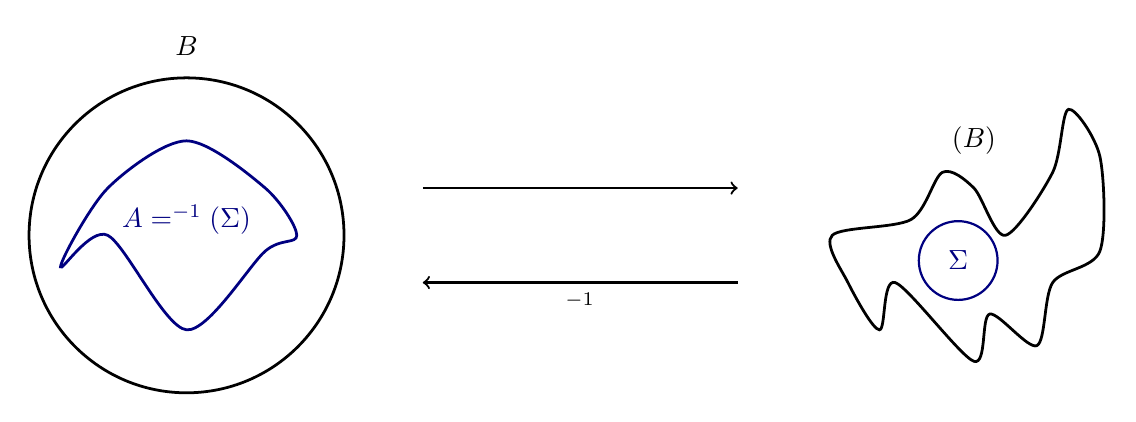
\begin{tikzpicture}[scale=2pt]
    \draw[thick,->] (-1,0.3)-- (1,0.3)%
    node[midway,above] {$\vphi$};
    \draw[thick,->] (1,-0.3) -- (-1,-0.3)%
    node[midway,below] {$\vphi^{-1}$}; 
    \draw[line width=1, black] (-2.5,0) circle (1);
    \draw node at (-2.5,1.2) {\color{black} $B$};
    \draw[line width=1, black] plot [smooth cycle, tension=0.5]%
    coordinates { (2.5,-0.8) (2.6,-0.5) (2.9,-0.7) (3,-0.3) (3.3,-0.1)% 
    (3.3,0.5) (3.1,0.8) (3,0.4) (2.7,0) (2.5,0.3) (2.3,0.4)%
    (2.1,0.1) (1.6,0) (1.7,-0.3) (1.9, -0.6) (2,-0.3)};
    \draw node at (2.5,0.6) {\color{black} $\vphi(B)$};

    \draw[thick, NavyBlue] (2.4,-0.16) circle (0.25);
    \draw node at (2.4,-0.16) {\color{NavyBlue} $\Sigma$};
    \draw[line width=1, NavyBlue] plot [smooth cycle, tension=0.5]%
    coordinates { (-2.5,-0.6) (-3, 0) (-3.3,-0.2) (-3,0.3) (-2.5,0.6)%
    (-2,0.3) (-1.8,0) (-2,-0.1)};
    \draw node at (-2.5,0.1) {\color{NavyBlue} $A=\vphi^{-1}(\Sigma)$};
  \end{tikzpicture}